% ------ APPENDIX A ------

\appendix
\chapter{User manual}
% ------ APPENDIX INTRO ------
This appendix explains how to correctly install and run the two implementations of the \oauth\ AuthZ Code Grant Flow: the former using as provider Google/Facebook and the latter using a custom AuthZ/Resource Server.
% ------ END OF APPENDIX INTRO ------

\minitoc

% ------ SECTION A.1 ------
\section{Software dependencies}
\label{appa}
Before installing and running the two implementations, there are some basic dependencies to install: \texttt{Docker} and \texttt{Docker-Compose}.

% ------ SECTION A.1.1 ------
\subsection{Docker}
\label{ublin}
The Docker Documentation \cite{docker} explains how to correctly install Docker on Windows/Ubuntu/macOS.

\paragraph{Ubuntu Linux (16.04 - 18.04 - 20.04)} First, all previous versions must be removed. 

\noindent From the bash terminal:
\begin{lstlisting}[language=bash]
  $ sudo apt-get remove docker docker-engine docker.io \
      containerd runc
\end{lstlisting}

\noindent Update and install packages to install dependencies over HTTPS:
\begin{lstlisting}[language=bash]
  $ sudo apt-get update
  $ sudo apt-get install \
      apt-transport-https \
      ca-certificates \
      curl \
      gnupg-agent \
      software-properties-common
\end{lstlisting}

\noindent Add Docker’s official GPG key:
\begin{lstlisting}[language=bash, showstringspaces=false, basicstyle=\ttfamily]
  $ curl -fsSL https://download.docker.com/linux/ubuntu/gpg | \ 
    sudo apt-key add -
\end{lstlisting}

\noindent Set-up the \textbf{stable} repository (change the \texttt{arch} param according to the architecture):
\begin{lstlisting}[language=bash, showstringspaces=false, basicstyle=\ttfamily]
  $ sudo add-apt-repository \
    "deb [arch=amd64] https://download.docker.com/linux/ubuntu \
    $(lsb_release -cs) \
    stable"
\end{lstlisting}

\noindent Install Docker:
\begin{lstlisting}[language=bash]
  $ sudo apt-get update
  $ sudo apt-get install docker-ce docker-ce-cli containerd.io
\end{lstlisting}

\noindent Add the current user to the \texttt{docker} group:
\begin{lstlisting}[language=bash]
  $ sudo groupadd docker
  $ sudo usermod -aG docker $USER
\end{lstlisting}

\noindent For different Linux distros or architectures, the Official Docs\footnote{\url{https://docs.docker.com/engine/install/}} is available.

\paragraph{Windows 10 Pro/Enterprise ($\geq Build 15063$)} The steps to follows are pretty straightforward:

\begin{itemize}
    \item[1.] Download Docker Desktop from the download page\footnote{\url{https://hub.docker.com/editions/community/docker-ce-desktop-windows/}}.
    \item[2.] Ensures that Hyper-V is enabled\footnote{\url{https://docs.microsoft.com/en-us/virtualization/hyper-v-on-windows/quick-start/enable-hyper-v}}.
    \item[3.] Double-click on the installer downloaded.
    \item[4.] Follow the standard installation procedure.
\end{itemize}

\paragraph{macOS ($\geq 10.13$)} Similarly to Windows:

\begin{itemize}
    \item[1.] Download Docker Desktop from the download page\footnote{\url{https://hub.docker.com/editions/community/docker-ce-desktop-mac/}}.
    \item[2.] Double-click on the \textit{.IMG} downloaded.
    \item[3.] Drag the application in the Application folder.
\end{itemize}
% ------ END OF SECTION A.1.1 ------

% ------ SECTION A.1.2 ------
\subsection{Docker-Compose}
For Windows and macOS systems, \texttt{docker-compose} is included in the Docker Desktop installation.\\
On Ubuntu Linux, the steps follow.

\noindent Install PIP:
\begin{lstlisting}[language=bash]
  $ sudo apt update
  $ sudo apt install python3-pip
\end{lstlisting}

\noindent Upgrade PIP:
\begin{lstlisting}[language=bash]
  $ sudo pip3 install -U pip
\end{lstlisting}

\noindent Install docker-compose:
\begin{lstlisting}[language=bash]
  $ sudo pip3 install docker-compose
\end{lstlisting}
% ------ END OF SECTION A.1.2 ------
% ------ END OF SECTION A.1 ------

% ------ SECTION A.2 ------
\section{Installation and use}
Once that \texttt{docker} and \texttt{docker-compose} are installed, the demos installation and use is not OS-dependent. Indeed, Docker Desktop (Windows/macOS) needs to be started as application first.

% ------ SECTION A.2.1 ------
\subsection{\oauth\ with Google/Facebook}
In order to install and run the implementation example that interacts with Google/Facebook, the file \texttt{docker-compose.yaml}\footnote{\url{https://github.com/nopesir/oauth-hw-security/releases}} is available in the resources as well as on GitHub as shown in Fig.~\ref{fig:rel1} (there are other files, but we only need the \texttt{.yaml} file).

\begin{figure}[h!]
    \centering
    \fbox{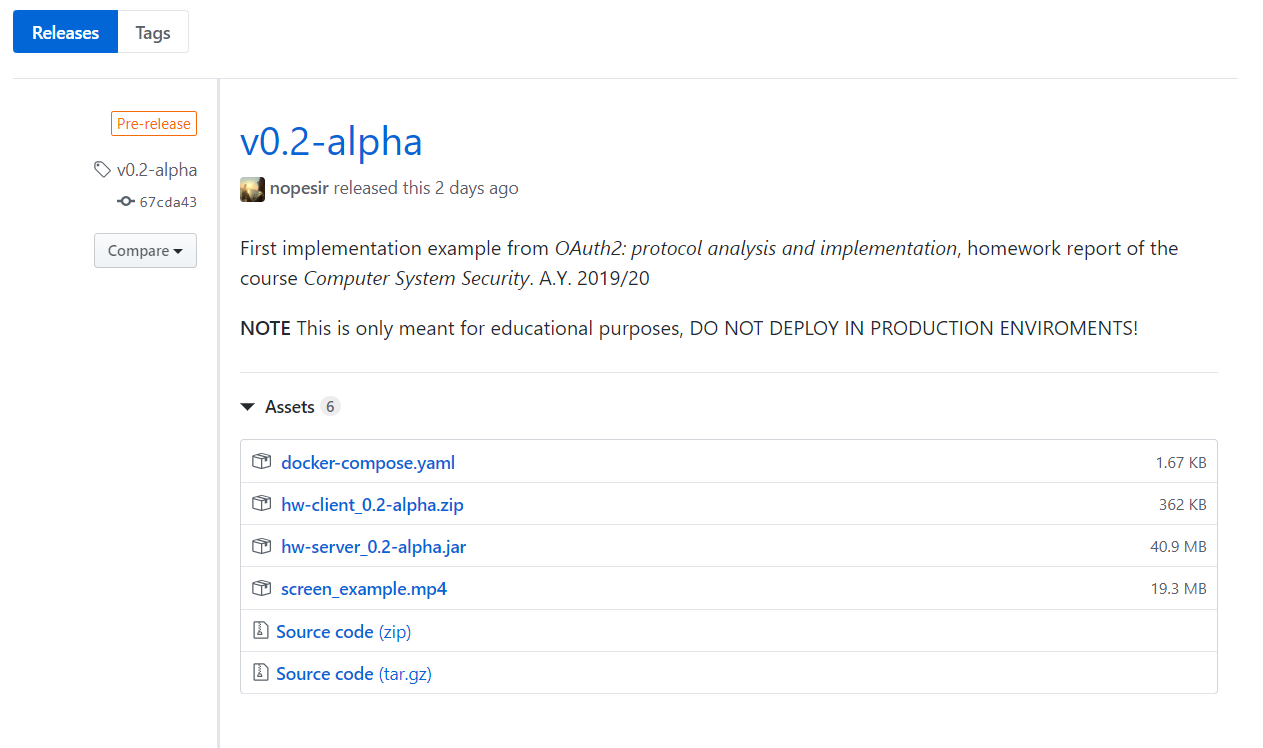
\includegraphics[scale=0.55]{chapters/images/chp5/release1.png}}
    \caption{GitHub Releases page: where to download the \texttt{docker-compose.yaml} file}
    \label{fig:rel1}
\end{figure}

\newpage

\noindent Then, in the same folder where \texttt{docker-compose.yaml} is, from the terminal:
\begin{lstlisting}[language=bash]
  $ docker-compose up
\end{lstlisting}

\noindent If all the dependencies are correctly installed and the docker daemon is running, \texttt{docker-compose} will automatically pull the containers, create the network namespace and start everything. The first run needs some time to download, but the next ones will use the downloaded data and will boot up the containers in a few seconds. The application now is running. From the browser, visit \texttt{http://localhost:9090} and the homepage will be displayed (Fig.~\ref{fig:home1}).

\begin{figure}[h!]
    \centering
    \fbox{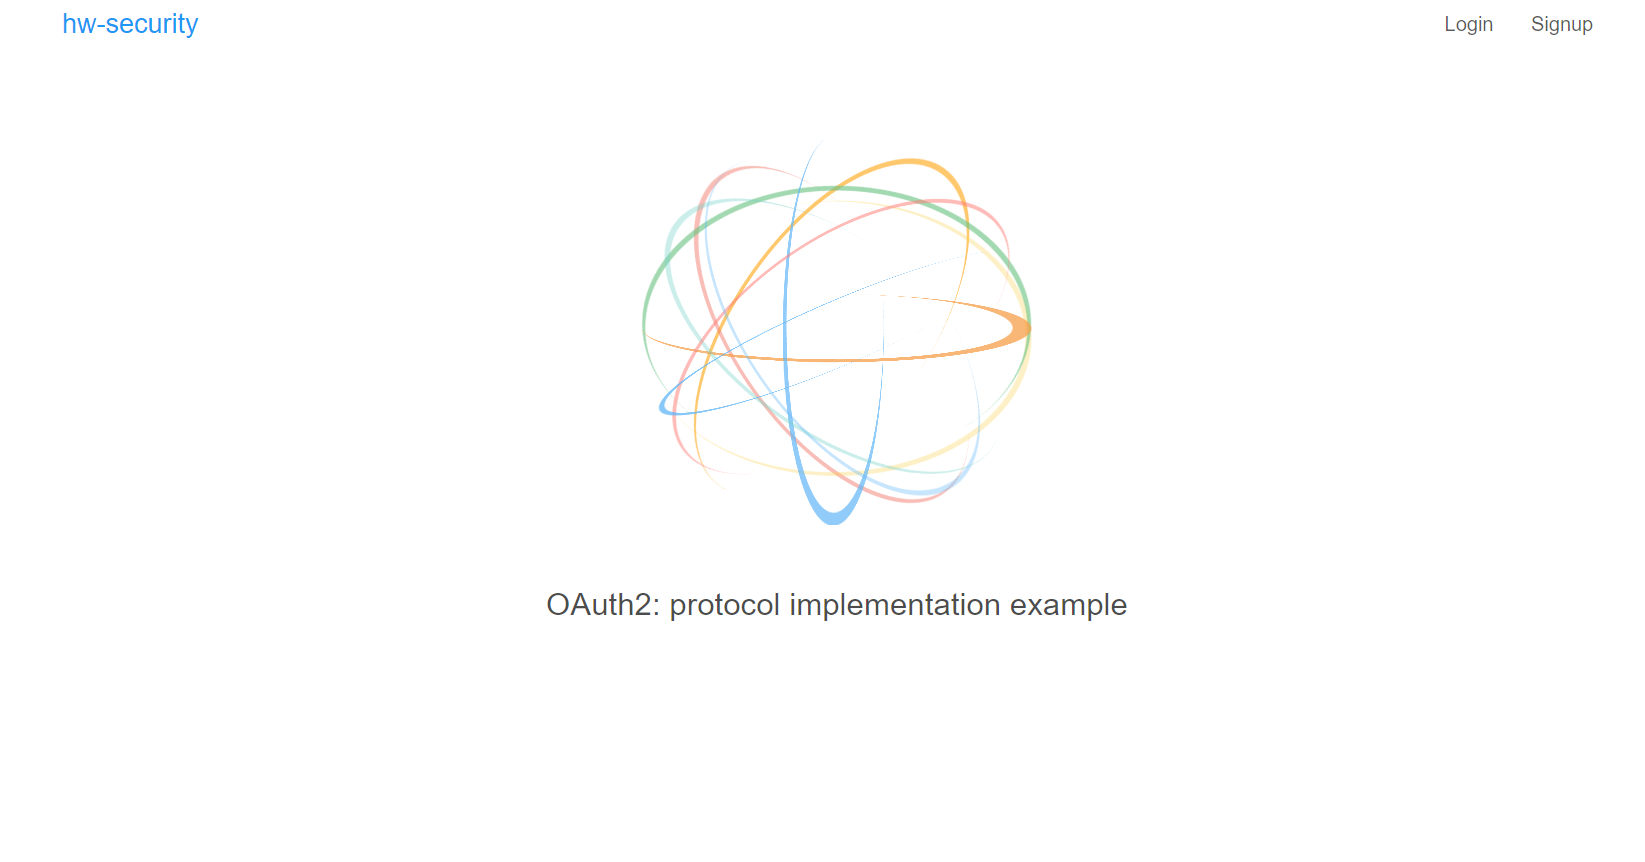
\includegraphics[scale=0.48]{chapters/images/chp5/screen1.png}}
    
    \caption{The homepage of the first implementation example}
    \label{fig:home1}
\end{figure}

\noindent To stop the application and safely detach all the resources, \texttt{Crtl+C} command on the terminal and finally a:
\begin{lstlisting}[language=bash]
  $ docker-compose down
\end{lstlisting}

\noindent The full screen video captioning of the example is available in the resources and in the Assets of the releases page\footnote{\scriptsize{\url{https://github.com/nopesir/oauth-hw-security/releases/download/v0.2-alpha/hw-security-screen.mp4}}}. 

\subsubsection{Troubleshooting}
\begin{itemize}
    \item Ensure to have ports \texttt{9090/tcp}, \texttt{8080/tcp} and \texttt{3306/tcp} available.
    \item Facebook login could give an error: Facebook App in test mode are accessible with \oauth\ only by the developer Facebook account\footnote{\url{https://developers.facebook.com/docs/apps/managing-development-cycle/\#step1}}, thus some test users must be added to the Facebook Developer's page. Use Google instead.
    \item Ensure to have at least 8GB of RAM on the machine.
    \item (Windows/macOS) Ensure that the Docker Desktop program is started.
    \item (Ubuntu Linux) Ensure that the Docker deamon is running.
\end{itemize}
% ------ END OF SECTION A.2.1 ------

% ------ SECTION A.2.2 ------
\subsection{\oauth\ with custom AuthZ/Resource servers}
In order to install and run the second example, the steps are almost the same as the previous subsection. The new \texttt{docker-compose.yaml} is available on the releases page\footnote{\url{https://github.com/nopesir/oauth-hw-security-custom/releases}} or in the resources (remove the previous \texttt{.yaml} file or choose another folder).

\noindent Then, in the same folder where \texttt{docker-compose.yaml} is, from the terminal:
\begin{lstlisting}[language=bash]
  $ docker-compose up
\end{lstlisting}

\noindent If all the dependencies are correctly installed and the docker daemon is running, \texttt{docker-compose} will automatically pull the containers, create the network namespace and start everything. 
The first run needs some time to download, but the next ones will use the downloaded data and will boot up the containers in seconds. The application now is running. From the browser, visit \texttt{http://localhost:9180} and the homepage will be displayed (Fig.~\ref{fig:home2}).

\begin{figure}[h!]
    \centering
    \fbox{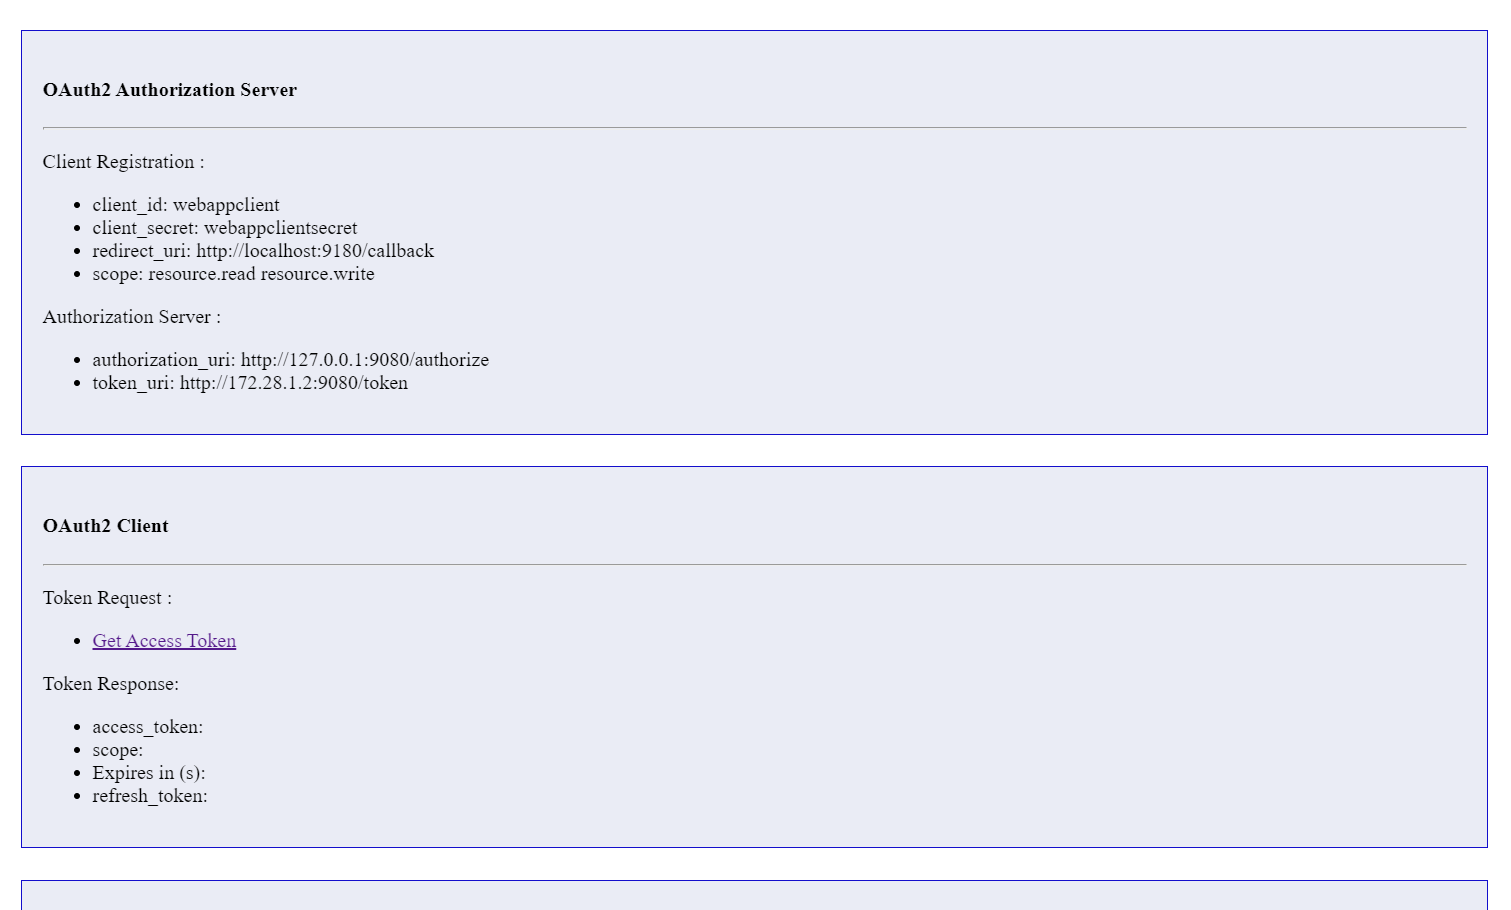
\includegraphics[scale=0.50]{chapters/images/chp5/screen2.png}}
    \caption{The homepage of the second implementation example}
    \label{fig:home2}
\end{figure}

\noindent Since this is an educational example, all the information are in plain text in the homepage. The first thing to do is to retrieve the access token by clicking on the link. Then, a log-in is necessary. The only available credentials are:

\begin{itemize}
    \item Username: \texttt{appuser}
    \item Password: \texttt{appusersecret}
\end{itemize}

\noindent After the log-in, it is displayed a checkbox in order to select what authorizations will be delegated to the client app. Select \texttt{resorce.read}, \texttt{resource.write} or both. 
Finally, the user will be redirected to the homepage with an access token. Now, it is time to request the resource using the two links at the end of the page. If the client is authorized, it will print a simple message, otherwise a 403 HTTP error is displayed (Forbidden). In addiction, it is available the refresh token flow based on the authorized resources or a subset of them (e.g. if someone has the access token for both scopes, it can make the token refresh for only one too). To stop the application and safely detach all the resources, \texttt{Crtl+C} command on the terminal and finally:
\begin{lstlisting}[language=bash]
  $ docker-compose down
\end{lstlisting}

\noindent The full screen video captioning of the example is available in the Assets of the releases page\footnote{\scriptsize{\url{https://github.com/nopesir/oauth-hw-security-custom/releases/download/v0.5-alpha/hw-security-custom-screen.mp4}}} or in the resources. 
% ------ END OF SECTION A.2.2 ------
% ------ END OF SECTION A.2 ------

% ------ END OF APPENDIX A ------